

\section{Motivating ReLU Dropping} \label{sec:Motivation}

In this section we motivate and present the key intuition behind ReLU dropping.  
We begin by defining the terms relevant to our discussion.

\begin{figure}[htbp] \centering
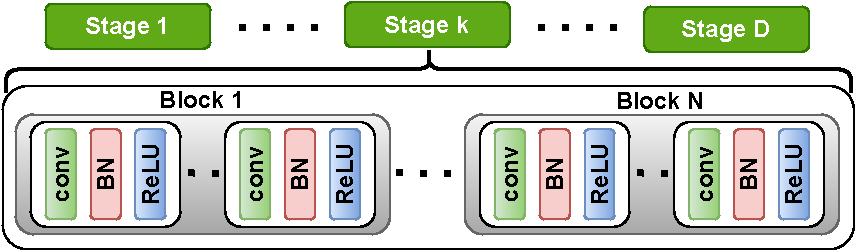
\includegraphics[scale=0.55]{Figures/NetHierarchy}
\vspace{-1em}
\caption{The structure of conventional ResNet-like architectures: %\cite{he2016deep,zagoruyko2016wide,
%xie2017aggregated,huang2017densely,huang2018condensenet,brendel2018approximating}.
Stages comprise Blocks and Blocks comprise multiple repetitions of conv, BN, and ReLU layers. 
%We follow this hierarchy in DeepReDuce in order to reduce the huge search space for ReLU optimization.
%this is the terminology we use to describe how ReLU dropping optimizations are applied.
}
\vspace{-1em}
\label{fig:NetHierarchy}
\end{figure}

\subsection{Notation}
Many state-of-art DNNs have a well defined hierarchy, 
which allows them to easily scale to different design points \cite{he2016deep,zagoruyko2016wide,xie2017aggregated,huang2017densely,huang2018condensenet,brendel2018approximating,sandler2018mobilenetv2}. 
These architectures consist of multiple Stages ($S$)
and each Stage contains copies of the same Block ($B$), as shown in Figure \ref{fig:NetHierarchy}. 
It is typical to call out the first convolution layer as Conv1, which we also do here.
The spatial resolution of the feature maps (fmaps) is same within a Stage. 
For example, the ResNet18 architecture contains four Stages, 
each with two residual Blocks where residual Blocks constitute
two $3\times3$ convolution layers \cite{he2016deep}.
Conventional scaling methods for designing smaller networks include 
channel and feature map scaling.
Channel scaling reduces the dimensions of the weights by a factor $\alpha$
and feature map scaling reduces the input resolution by $\rho$~\cite{howard2017mobilenets,tan2019efficientnet}.

When describing a DeepReDuce optimized network we explicitly name stages with ReLUs intact.
E.g., $S_{2} + S_{3}$ implies stages $S_1$ and $S_4$ have their ReLUs completely removed and
only $S_2$ and $S_3$ have ReLUs.
When a stage is optimized with \textit{ReLU Thinning} (see below for details)
we superscript it with $RT$, e.g., $S_2^{RT}$.
When channel and feature maps' resolution scaling are applied we specify $\rho$ and $\alpha$ amounts.
%\fixme{This is not consistent with algorithm1.}
 \begin{table} [t]
\caption{ReLUs' criticality evaluation: ReLU counts and accuracy (CIFAR-100) for ResNet models
where ReLUs are dropped from all but one stage. 
%E.g., S1 indicates the only network ReLUs are in S1.
We posit that less accurate ReLU stages indicate less important
ReLUs and note accuracy differs significantly across stages.}
\label{tab:ReluHeteroR18}
\centering 
\resizebox{0.49\textwidth}{!}{
\begin{tabular}{cccccccc} \toprule
Models & Metrics & No ReLUs & Conv1 & $S_1$ & $S_2$ & $S_3$ & $S_4$ \\ \toprule
\multirow{3}{*}{ ResNet18 } & \#ReLUs & 0 & 66K & 262K & 131K & 66K & 33K \\
& W/o KD (\%) & 18.49 & 46.22 & 61.93 & 67.63 & 67.41 & 58.90 \\
& W/ KD (\%) & 18.34 & 45.07 & 59.85 & 68.79 & 69.92 & 63.16 \\ \midrule
\multirow{3}{*}{ResNet34} & \#ReLUs & 0 & 66K & 393K & 262K & 197K & 49K \\
& W/o KD(\%) & 18.16 & 45.42 & 60.77 & 69.47 & 70.04 & 57.44 \\
& W/ KD(\%) & 18.07 & 45.13 & 62.88 & 70.93 & 72.61 & 64.23 \\
\bottomrule
\end{tabular} }
\end{table}



\subsection{ReLU Dropping}
We now discuss four observations motivate ReLU dropping and DeepReDuce.


\begin{figure}[t]
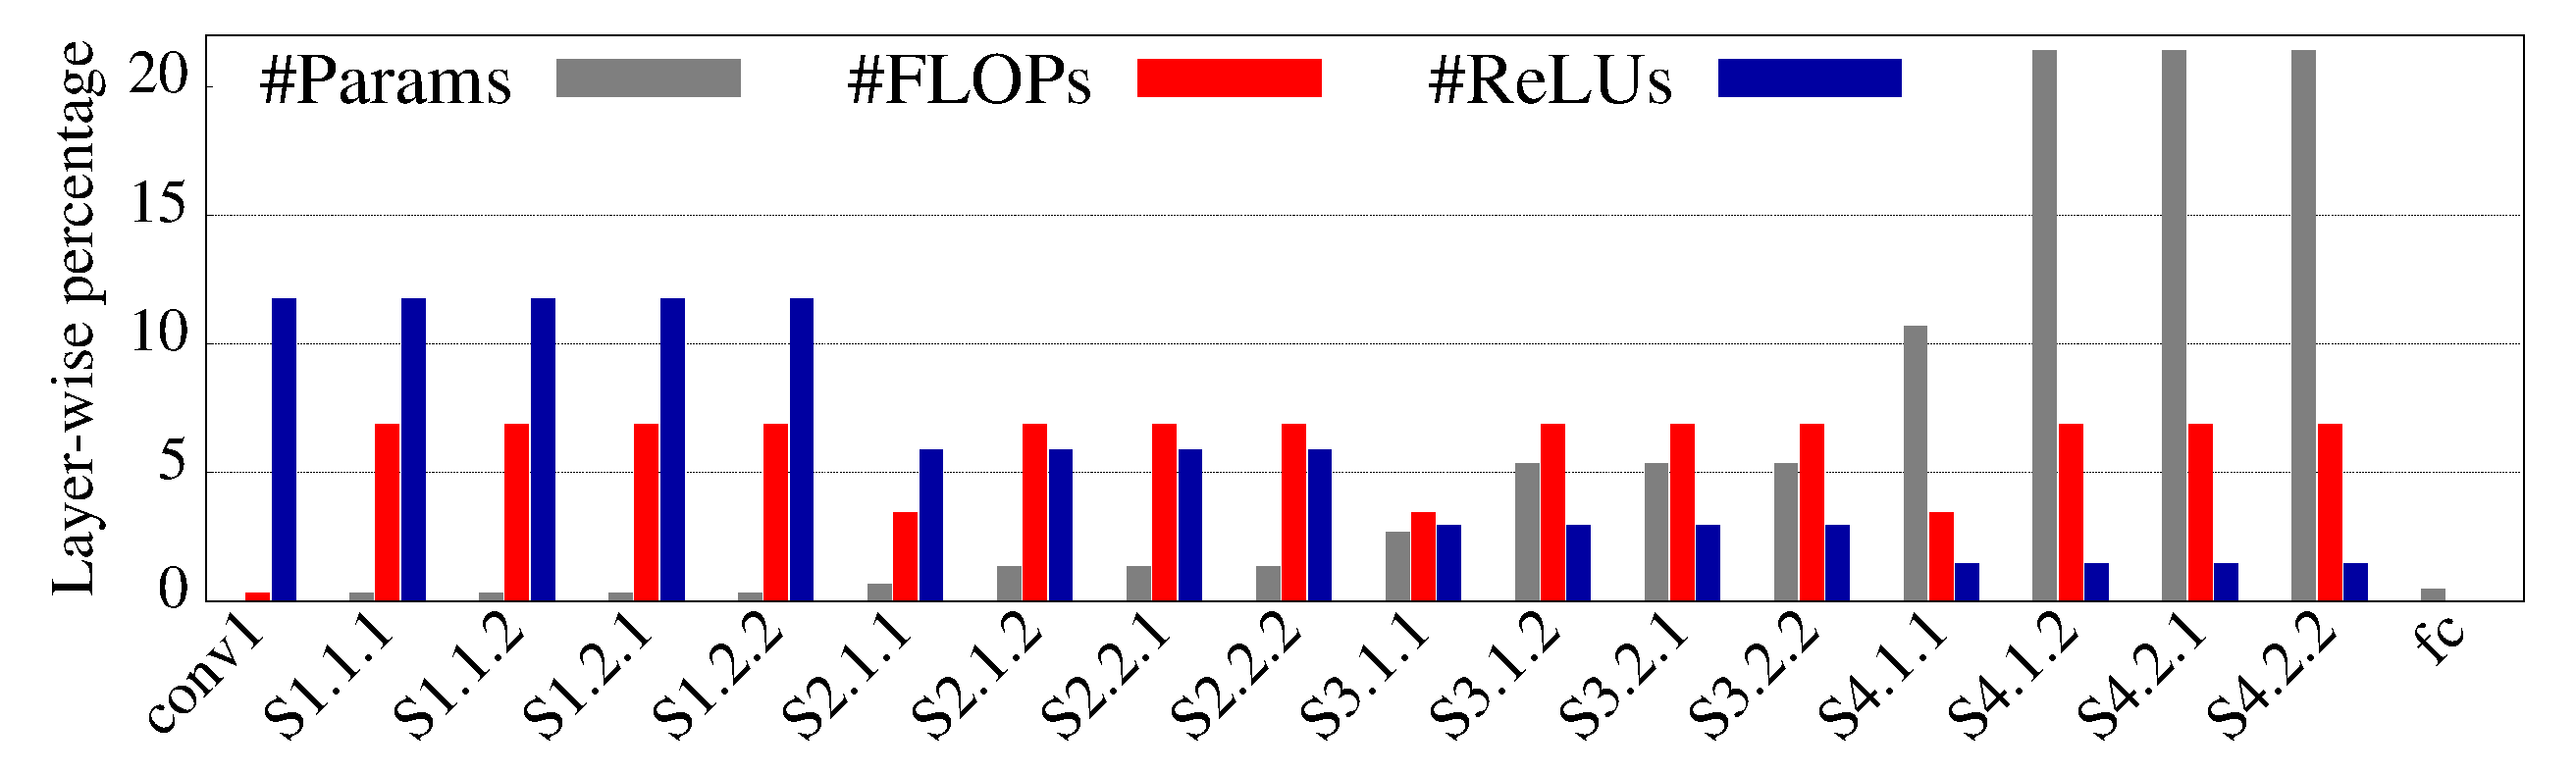
\includegraphics[scale=0.19]{Figures/LayerWiseOps_R18}
\vspace{-2em}
%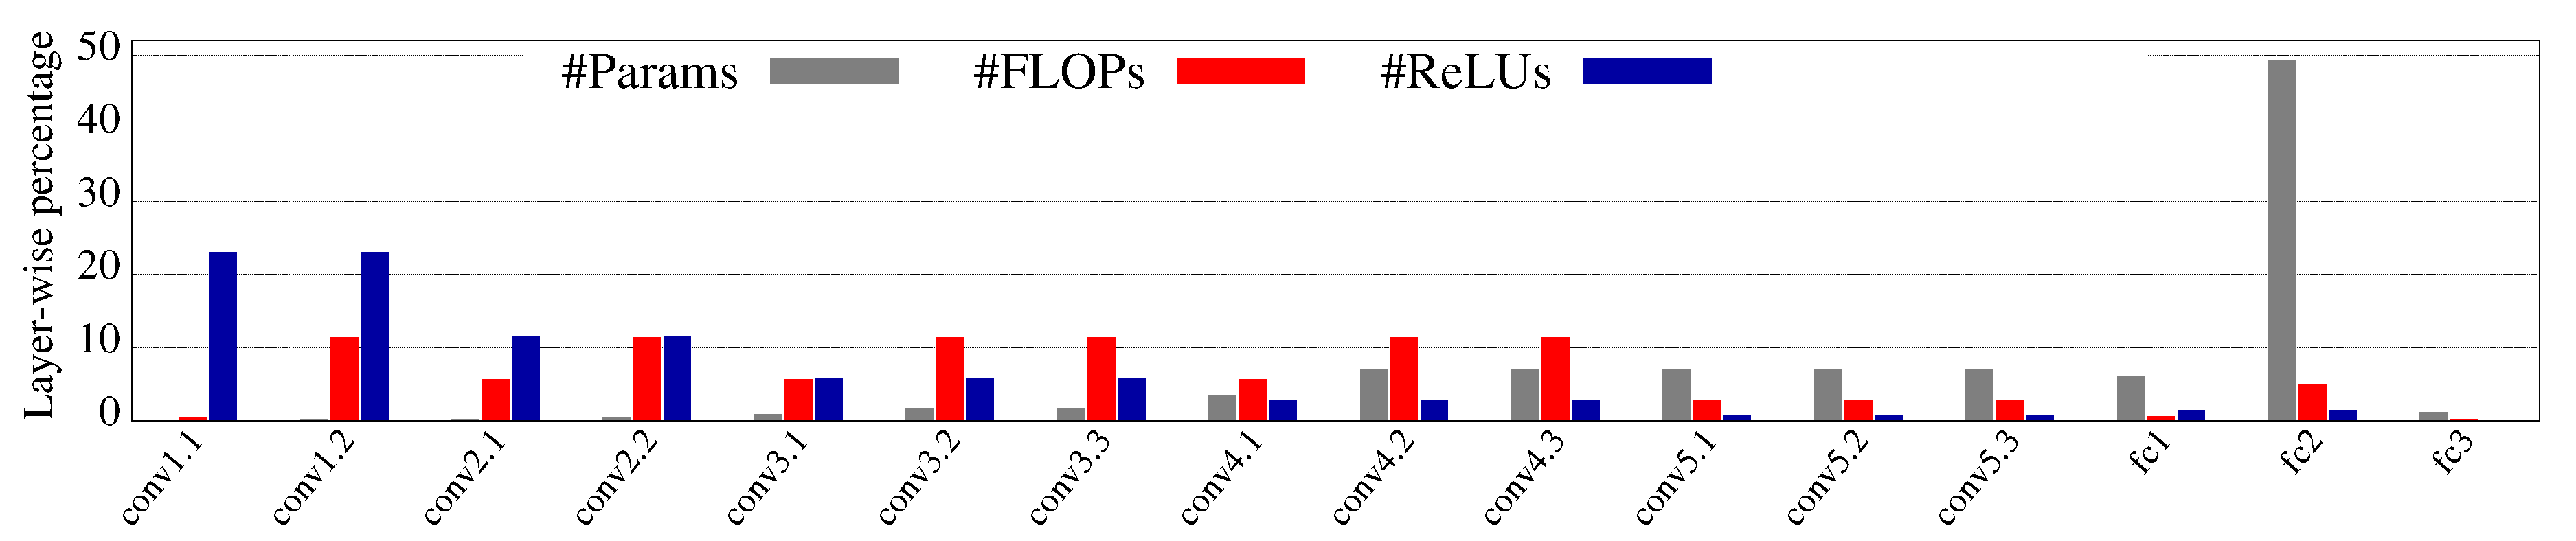
\includegraphics[scale=0.2]{Figures/LayerWiseOps_Vgg16} \\
%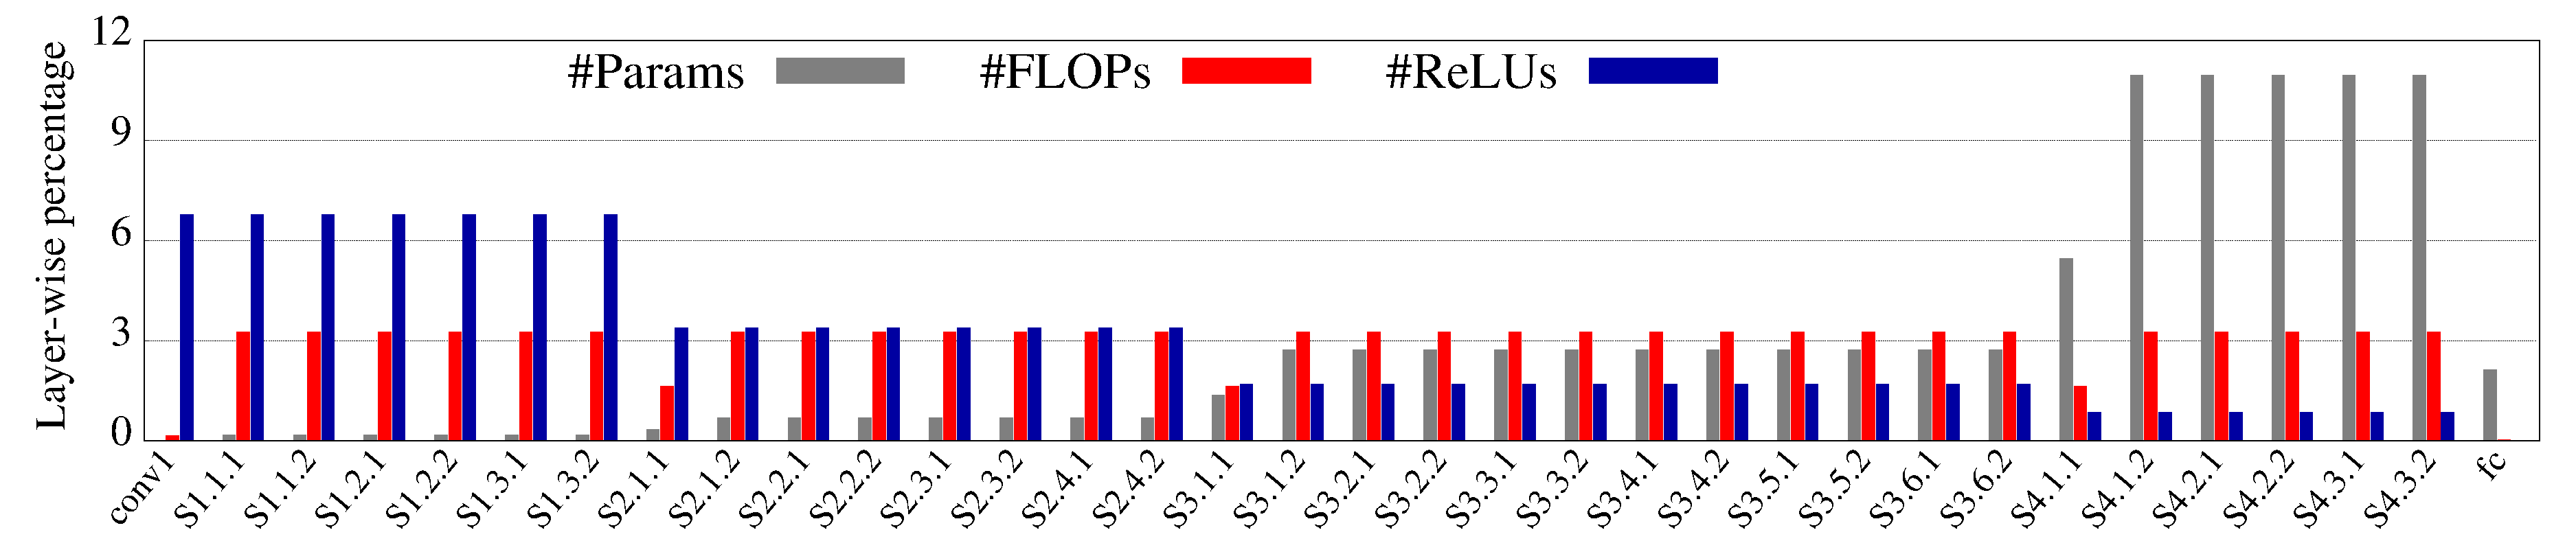
\includegraphics[scale=0.2]{Figures/LayerWiseOps_R34} 
%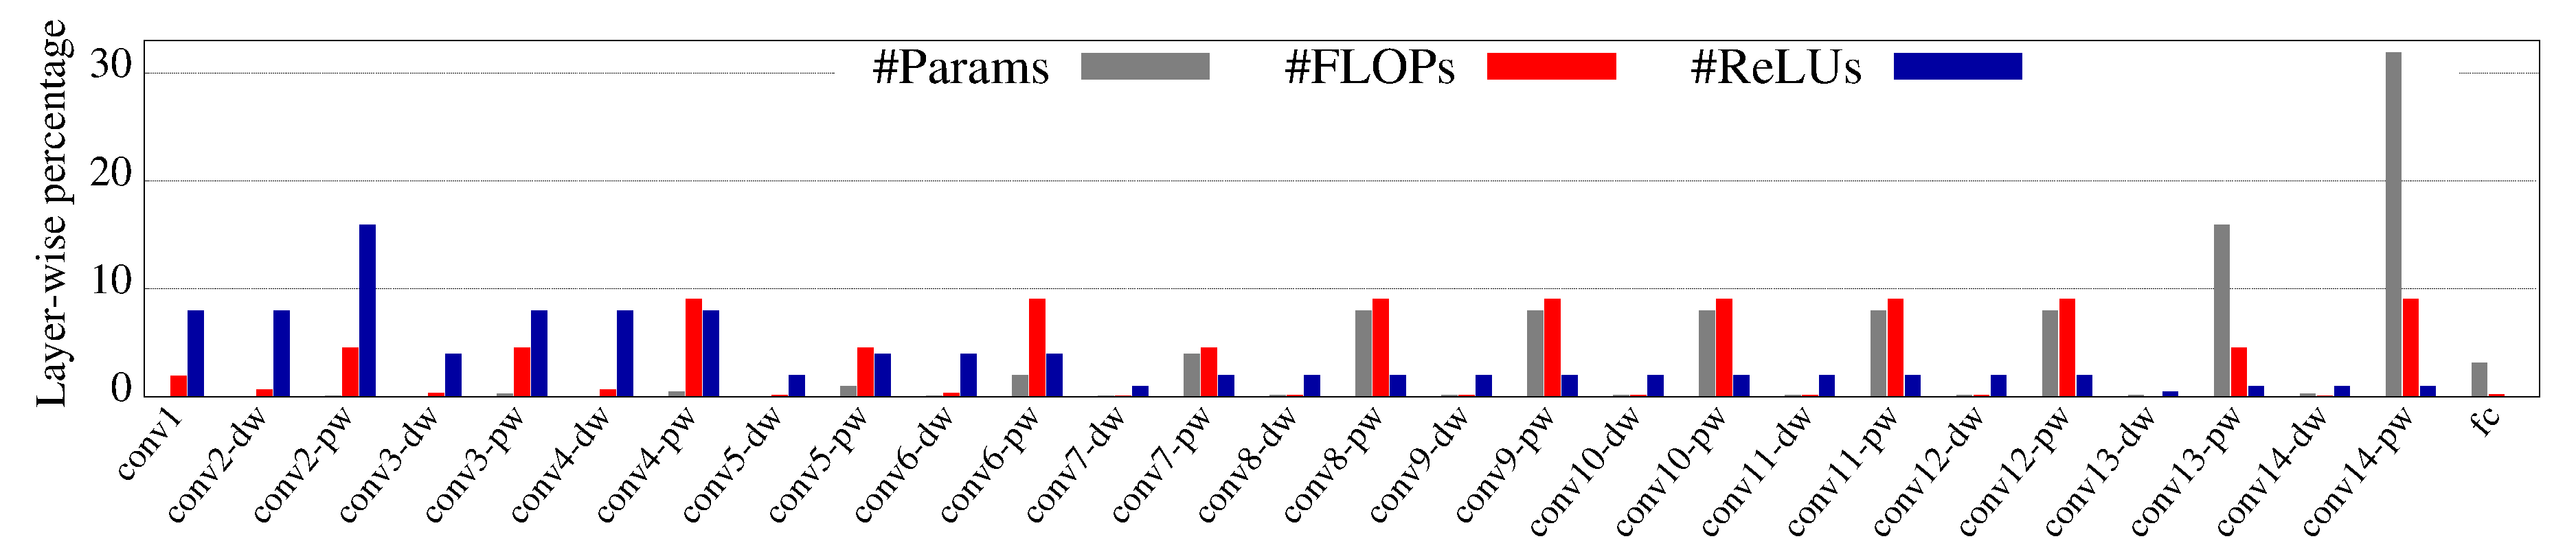
\includegraphics[scale=0.2]{Figures/LayerWiseOps_MV1} \\
%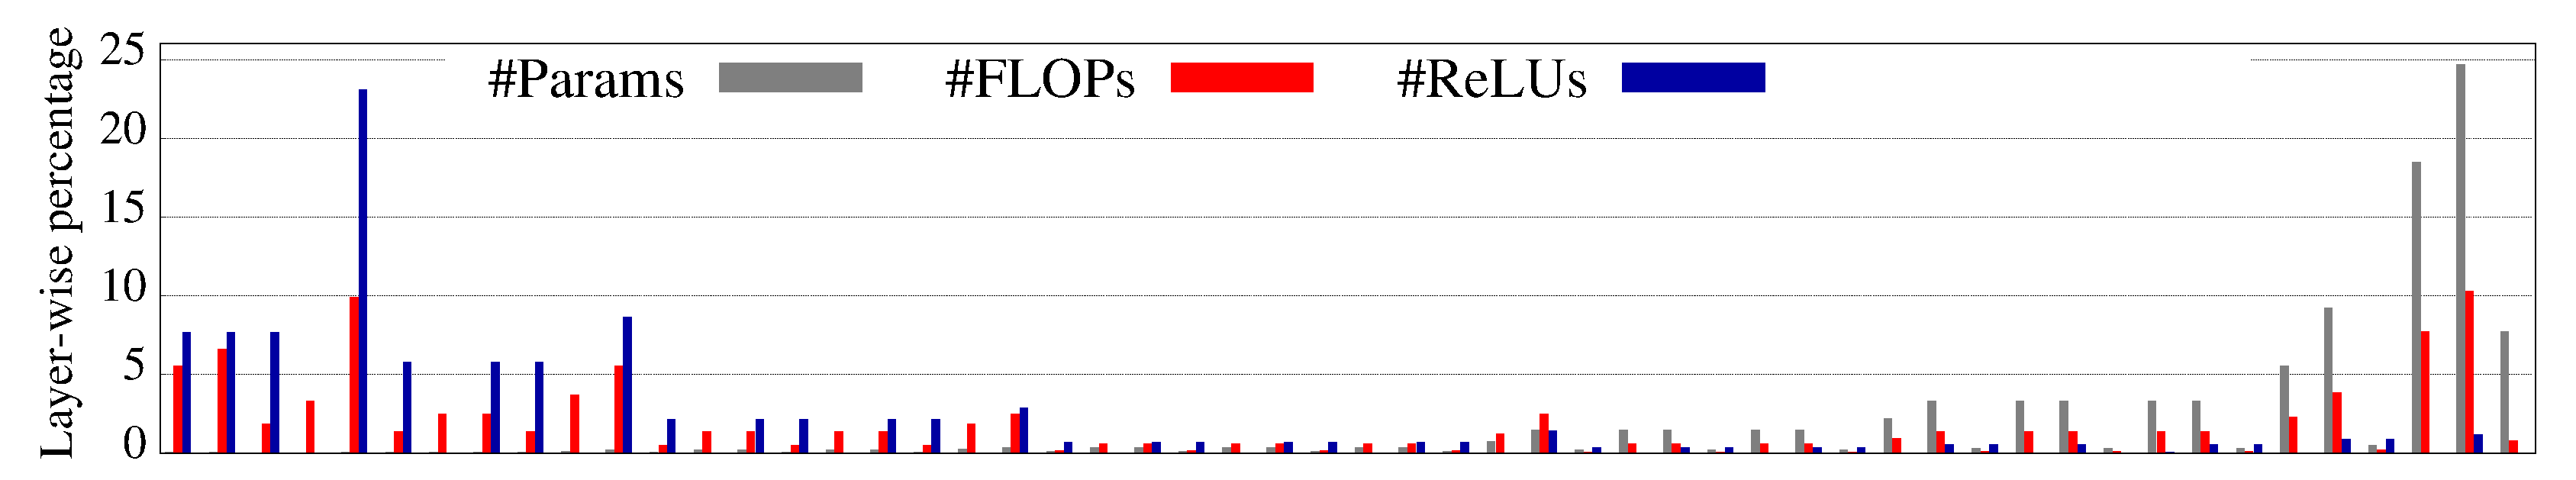
\includegraphics[scale=0.32]{Figures/LayerWiseOps_MV2}
\caption{
Layer-wise distribution of parameters, FLOPs, and ReLUs in ResNet18.
FLOPs are evenly distributed, parameters (ReLUs) are increases (decreases) with network's depth.} 
\label{fig:LayerWiseReluInDNNs}
\vspace{-1em}
\end{figure}

\textbf{Observation 1: ReLUs are unevenly distributed across
the layers of conventional CNNs.} 
We begin by investigating the distribution of ReLUs across the layers of modern CNN architectures. 
Figure~\ref{fig:LayerWiseReluInDNNs} presents a layer-wise breakdown
of ResNet18's ReLUs, FLOPS, and parameters.
We observe that FLOPs are evenly distributed across layers,
and that the number of ReLUs per layer decreases with depth while 
the parameter count increases with depth.
A similar distribution of parameters, FLOPs, and ReLUs have
been observed in other common CNNs
(Figure \ref{fig:LayerWiseReluInOtherDNNs} in  Appendix \ref{secAppendix:LayerWiseOpsInDNNs}).

The skewed distribution of ReLUs is because
conventional CNN architectures
tend to scale the number of channels up by $2\times$ and the fmap spatial dimension down by $2\times$ in \emph{each} dimension across stages, 
resulting in a $2\times$ drop in ReLU count across a down-sampling layer.
All other Things being equal, this presents an opportunity to significantly reduce
ReLU counts by simply dropping them from early stages.
This fortuitous as we also observe
ReLUs in the early stages tend to be less critical for accuracy.


\textbf{Observation 2: ReLUs in some stages are more 
important for accuracy than others.}
To understand the relative importance of ReLUs in different network stages
we crafted ablation experiments.
This was done by removing ReLUs from all but one ResNet18 stage
and training each resulting network from scratch.
Table~\ref{tab:ReluHeteroR18} shows the accuracy and ReLU count of each resulting network
using the CIFAR-100 dataset. 
Recall that ResNet18 has Conv1 layer prior to stage 1.
For completeness (in Table~\ref{tab:ReluHeteroR18}) we report result for ResNet18 with ReLUs only in Conv1.  However, we always drop ReLUs from Conv1 along with stages in the network in subsequent experiments.

We note that the four resulting networks vary greatly with respect to accuracy. 
Networks with ReLUs in $S_2$ and $S_3$ (Table \ref{tab:ReluHeteroR18}) have high accuracy, 
even though $S_2$ and $S_3$ use fewer ReLUs than $S_1$. 
Similarly, although Conv1 and $S_3$ have the same number of ReLUs, 
allocating ReLUs to $S_3$ instead of Conv1 increases accuracy by 24.8\%. 
A similar ReLU-accuracy disparity was observed for ResNet34 (see Table~\ref{tab:ReluHeteroR18}.) 
We conclude that not all ReLUs are equal:
some contribute more to model accuracy than others.
We hypothesize these less important ReLUs can be removed without significantly impacting network's accuracy.


{\bf Observation 3: Some ReLUs benefit more from knowledge distillation that others.}
Given the disparate impact of dropping ReLUs from stages in a network, 
we also investigated whether some stages benefit more from KD than others. 
As illustrated in the Table~\ref{tab:ReluHeteroR18}, 
the accuracy gain from KD is position dependent and greater for networks with ReLUs in deeper stages ($S_4$ and $S_3$) compared to the networks with ReLUs in initial stages ($S_1$ and $S_2$).
Our results thus suggest that KD is synergistic with ReLU dropping:
dropping ReLUs from early layers dramatically reduces ReLU count with a relatively small impact on accuracy and would not have benefited as much from KD had ReLUs in these layers been preserved.
Conversely, latter layers with a small number of more critical ReLUs also benefit the most from KD. 
This resonates with the claim made in~\cite{gotmare2018a}
as knowledge shared by a teacher in KD is primarily disbursed in deeper layers.
 
%are the easiest to drop, have the most ReLUs, and are ill-suited for 
%KD while later layers have fewer ReLUs and work well with KD.


\begin{table} [t]
\caption{
Performance comparison of channel scaling ($\alpha$=0.5) and dropping ReLUs 
from alternate layers (S$_k^{RT}$ where $k$ is the network stage) using ResNet18 on CIFAR-100. 
Both methods reduce ReLUs by a factor of 2$\times$; 
however, alternate ReLU dropping results in more accurate iso-ReLU networks.}
\label{tab:AlphaVsReluDrop}
\centering 
\resizebox{0.49\textwidth}{!}{
\begin{tabular}{ccccc} 
 \toprule
 Network & \#Conv & \#ReLUs & W/o KD(\%) & W/ KD(\%) \\ \toprule
%\multirow{1}{*}{\bf Network } & \multirow{1}{*}{\bf \#Conv } & \multirow{1}{*}{\bf \#ReLU } & \multicolumn{2}{c}{\bf CIFAR-100 } \\
%& & & {\bf w/o kD} & {\bf w/ KD} \\
 
$S_{2}$+$S_{3}$+$S_{4}$  & 17 & 229K & 73.14 & 76.22 \\
$S_{2}^{RT}$+$S_{3}^{RT}$+$S_{4}^{RT}$ & 17 & 115K & 72.97 & 74.72 \\
$S_{2}$+$S_{3}$+$S_{4}$, $\alpha$=0.5 & 17 & 115K & 71.59 & 73.78 \\ \midrule
%$Arch2$ $\rightarrow$ Res18(FR) - relu[conv1 + S1] & 11 & 115K & 71.96 &	74.57 \\ 
$S_{2}$+$S_{3}$  & 17 & 197K & 72.77 & 75.51 \\
$S_{2}^{RT}$+$S_{3}^{RT}$ & 17 & 98K & 70.97 & 71.95 \\
$S_{2}$+$S_{3}$, $\alpha$=0.5 & 17 & 98K & 69.54 & 71.16 \\ \midrule
%$Arch2$ $\rightarrow$ Res18(FR) - relu[conv1 + S1 +S4] & 13 & 98K & 70.15 &	72.17 \\ \midrule
$S_{3}$+$S_{4}$ & 17 & 98K & 68.4 & 73.16 \\
$S_{3}^{RT}$+$S_{4}^{RT}$ & 17 &49K & 69.62 & 71.06 \\
$S_{3}$+$S_{4}$, $\alpha$=0.5 & 17 & 49K & 66.43 & 70.29 \\ 
%$Arch2$ $\rightarrow$ Res18(FR) - relu[conv1 + S1 + S2] & 13 & 49K & 66.68 &	69.79 \\
\bottomrule
\end{tabular}} 
\vspace{-1.5em}
\end{table}



\textbf{Observation 4: Dropping ReLUs within stages is better than channel scaling.}
Our final observation relates to the relative importance of ReLUs \emph{within} network 
stages. 
We explore two strategies for $2\times$ ReLU reduction in a stage: 
(i) drop ReLUs from alternate layers or 
(ii) reduce the number of channels in the stage by $2\times$.
Table~\ref{tab:AlphaVsReluDrop} compares alternate layer ReLU dropping against channel down scaling for three different network architectures obtained by dropping ReLUs in $S_1$, $S_1+S_4$, and $S_1+S_2$.
In each instance we observe that at iso-ReLU, alternate layer ReLU dropping has $1\%-3\%$ accuracy improvements over channel down-scaling. 
We note that even with KD
alternate layer ReLU dropping is consistently better than channel down-scaling.